\documentclass{subfiles}

\begin{document}


    \begin{Frage}
        Licht- Materie Wechselwirkung (Absorbtion und Emission).
    \end{Frage}
    \begin{Antwort}
        Es gibt hier im Groben drei interessante Fälle. Betrachte zunächst das Schaubild:
        \begin{figure}[H]
            \centering
            \includegraphics[width=8cm]{Bilddateien/AbsorptionEmission.png}
            \caption{Schematische Darstellung der Absorbtion und Emission von Licht durch ein Atom \cite{exp8-paper}.}
            \label{fig:AbsorptionEmission}
        \end{figure}
        \begin{enumerate}
            \item Die \emph{Absorbtion} von Licht durch ein Atom. Es liegt eine Proportionalität $\dv{t}N(t)\propto n_1\cdot u_{ph}$ vor, wobei $u_{ph}$ die Photonenenergiedichte ist. Der Proportionalitätsfaktor ist die \emph{Absorbtionsrate} $B_{1\to 2}$ (Einstein Koeffizient).
            \item Die \emph{induzierte Emission} von Licht durch ein Atom. Es liegt eine Proportionalität $\dv{t}N(t)\propto n_2\cdot u_{ph}$ vor, wobei der Proportionalitätsfaktor hier die \emph{induzierte Emissionsrate} $B_{2\to 1}$ ist.
            \item Die \emph{spontane Emission} von Licht durch ein Atom. Es herrscht hier eine Proportionalität $\dv{t}N(t) \propto n_2\cdot V$. 
        \end{enumerate}
        Man kann hier zeigen, daß $B_{1\to 2} = B_{2\to 1}$ gilt. 
        \begin{figure}[H]
            \centering
            \begin{subfigure}[t]{0.4\textwidth}
                \centering
                \includegraphics[width=\textwidth]{Bilddateien/StimulatedEmission.png}
                \caption{Induzierte Emission.}
                \label{fig:StimulatedEmission}
            \end{subfigure}
        \end{figure}
        Über die spontane Emission kann weiter eine \emph{Lebensdauer} $\tau$ definiert werden, welche die Lösung der vorgestellten Differentialgleichung der Form 
        \[
            n_2(t) = n_2(0)\cdot \exp(-A_{2\to 1}\cdot t)
        \]
        mit $\tau = 1/A_{2\to 1}$ ist. \\

        Die \emph{spektrale Linienbreite}, also der Energiewert, bei welchem spontane Absorbtion stattfindet, ist gegeben durch $\Delta E\cdot\delta t \geq \hbar/2$. Die Absorbtionslinie ist also nicht scharf, sondern folgt einer Gaußkurve mit Breite $\Delta E$:
        \begin{figure}[H]
            \centering
            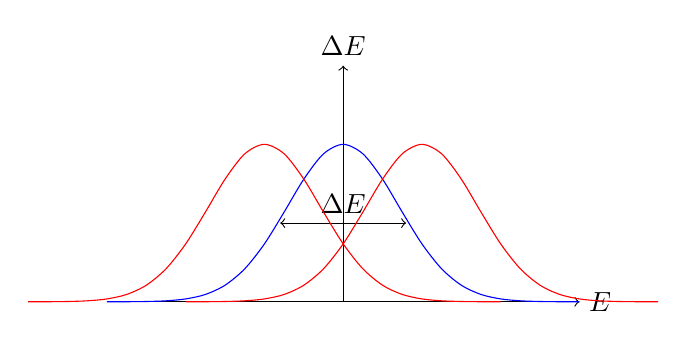
\begin{tikzpicture}
                \draw[->] (-3,0) -- (3,0) node[right] {$E$};
                \draw[->] (0,0) -- (0,3) node[above] {$\Delta E$};
                \draw[domain=-3:3,smooth,variable=\x,blue] plot ({\x},{2*exp(-\x*\x)});
                \draw[<->] (-0.8,1) -- (0.8,1) node[midway,above] {$\Delta E$};

                % draw overlapping gauusian curves displaced by +- 1
                \draw[domain=-3:3,smooth,variable=\x,red] plot ({\x-1},{2*exp(-\x*\x)});
                \draw[domain=-3:3,smooth,variable=\x,red] plot ({\x+1},{2*exp(-\x*\x)});
            \end{tikzpicture}
            \caption{Spektrale Linienbreite. Einzelner Peak in blau, mögliche Überlagerung in rot. Siehe FWHM.}
        \end{figure}
    \end{Antwort}

    \begin{Frage}
        Wie funktioniert ein Laser?
    \end{Frage}
    \begin{Antwort}
        Am Beispiel eines vier Niveau Lasers. 
        \begin{figure}[H]
            \centering
            \includegraphics[width=8cm]{Bilddateien/Lasing.svg.png}
            \caption{Schematische Darstellung eines Vier-Nievau-Lasers am Beispiel stimulierter Emission.}
            \label{fig:Lasing}
        \end{figure}
        Voraussetzung für die Funktionalität ist eine Schnelle Relaxation von $E_P$ und eine kurze Lebensdauer von $E_L$. Die Anregung von $E_0$ muss dabei schneller sein als die Relaxation von $E_L$ zu $E_0$, um eine Besetzungsinversion stationär zu erreichen. Betrachte nun die Prozesse bei $E_M$ als entscheidendes Niveau. 
        \begin{align*}
            \dv{t}N_{E_M}^{(P)}(t) = \eta\cdot W_{1\to 4}\cdot N_{E_1}(t), \tag{P}
        \end{align*}
        wobei $\eta$ die Pumpeffizienz angibt. Dabei nehmen wir die sehr schnelle Entvölkerung von $E_P$ an: $N_{E_P} \approx 0$. 
        \[
            \dv{t}N_{E_M}^{(S)}(t) = -\frac{1}{\tau_S}\cdot N_{E_M}^{(S)}(t). \tag{S}
        \]
        Hierbei ist $\tau_S$ die Lebensdauer von $E_M$, siehe oben. 

        Es kann jedoch ebenfalls zwischen $E_M$ und $E_L$ eine induzierte Absorbtion stattfinden:
        \[
            \dv{t}N_{E_M}^{(I)}(t) \propto p\cdot (N_{E_L}^{(I)}(t) - N_{E_M}^{(I)}(t)). \tag{I}
        \]
        Dabei ist $p$ die Photonendichte des herrschenden Laserfeldes um das Atom herum. Sei $k$ hier die Proportionalitätskonstante, dann gilt im Summation
        \[
            \dv{t}N_{E_M}(t) = \eta\cdot W_{1\to 4}\cdot N_{E_1}(t) - \frac{1}{\tau_S}\cdot N_{E_M}(t) + k\cdot (N_{E_L}(t) - N_{E_M}(t)).
        \]

        Für die Photonendichte erhält man dann 
        \[
            \dv{t}p(t) = p(t)\cdot\nbra{k\cdot n - \frac{1}{\tau_{ph}}}.
        \]

        \subsubsection*{Statische Lösungen}
        Da praktisch jedoch weder Pumprate, noch Photonendichte messbar sind, verlassen wir uns auf die Output-Leistung $P_o$ als Funktion der Inputleistung $P_p$ mit einer Grenze $P_{th}$, ab welcher der Laser zu leuchten beginnt:
        \[
            P_a(P_p) = \alpha_S\cdot (P_p - P_{th}), \tag{P}
        \]
        wobei hier der lineare Zusammenhang relevant ist und $\alpha_S = \eta\cdot E_{3,2}/E_{4,1} \cdot T/(T + L)$ die Steigungseffizienz mit folgenden Parametern ist:
        \begin{itemize}
            \item $\eta$ die Pumpeffizienz,
            \item $T$ die Transmission des Resonators,
            \item $L$ die Verluste des Resonators,
            \item $E_{3,2}$ die Energiedifferenz zwischen $E_3$ und $E_2$ und
            \item $E_{4,1}$ die Energiedifferenz zwischen $E_4$ und $E_1$.
        \end{itemize}
        Der Quotient $E_{3,2}/E_{4,1}$ heißt \emph{quantum efficiency}.
        Als Funktion sieht das ganze dann so aus:
        \begin{figure}
            \centering
            \includegraphics[options]{Bilddateien/Pumpleistung.png}
            \caption{Outputleistung als Funktion der Inputleistung.}
            \label{fig:Pumpleistung}
        \end{figure}
        Beim Laserbau muss ebenfalls nach $T$ und $L$ optimiert werden, wodurch sich jedoch die Output Leistung reduziert. 
        \begin{figure}[H]
            \centering
            \includegraphics[width=8cm]{Bilddateien/TOptimierung.png}
            \caption{Optimierung der Outputleistung durch Variation der Transmission $T$.}
        \end{figure} 

        \subsubsection*{Variierende Lösungen}
            Als ersten Kontakt mit nichtstatischen Lösungen betrachten wir das Einschalten der Pumpe. Bis zum Erreichen von $P_{ph}$ gibt es quasi keine angeregten Nd Atome. Ab diesem Punkt wird jedoch ein Photonenfeld $p(t)$ erzeugt, wodurch die Änderungsrate von $p$ groß wird. 

    \end{Antwort}

    \begin{Frage}
        Optische Resonatoren.
    \end{Frage}
    \begin{Antwort}
        Grundätzlich unterscheiden wir zwischen \emph{planparallelen}, \emph{hemispheärischen} und \emph{sphärischen} Resonatoren.
        \begin{figure}[H]
            \centering
            \includegraphics[width=8cm]{Bilddateien/ResonatorBasic.png}
            \caption{Schematische Darstellung eines optischen Resonators \cite{exp8-paper}.}
            \label{fig:OptischerResonator}
        \end{figure}
        Zur Stabilität lassen sich für gegebene Krümmungsradien $R_1$ und $R_2$ die \emph{Gaußschen Resonatorparameter} $g_1$ und $g_2$ definieren:
        \[
            g_1 = 1 - \frac{L}{R_1}, \qquad g_2 = 1 - \frac{L}{R_2}.
        \]
        Die Abbildung zeigt dann das Stabilitätsgebiet mit $g_1\cdot g_2\in [0,1]$.
        \begin{figure}[H]
            \centering
            \includegraphics[width=8cm]{Bilddateien/StabileGebiete.png}
            \caption{Stabilitätsgebiete für optische Resonatoren.}
            \label{fig:StabileGebiete}
        \end{figure}
        In diesem Resonator können sich nun stehende Wellen ausbilden, welche durch die \emph{Resonatormoden} beschrieben werden. Die Moden sind dabei durch die \emph{Resonatorlänge} $L$ und die Lichtwellenlänge $\lambda$ gegeben; Lösungen sind $\lambda_n/2\in\N$ mit 
        \[
            \frac{\lambda_n}{2}= \frac{L}{n}\implies \lambda_{n+1} - \lambda_n = \frac{2L}{n\cdot (n+1)} = \frac{c}{2\cdot L}.  
        \]
        Im Beispiel des NdYAG Lasers können demnach bei $L = 50\si{\mm}$ und $\Delta\lambda = 3\si{\giga\hertz}$ etwa $n = 30$ Moden auftreten mit $\lambda = 1064\si{\nano\meter}$.
    \end{Antwort}

    \begin{Frage}
        Lasertypen.
        \begin{itemize}
            \item Halbleiterlaser (Beispiel AlGaAs)
            \item Festkörperlaser (Beispiel Nd:YAG)
        \end{itemize}
    \end{Frage}
    \begin{Antwort}
        \subsection*{Aluminium-Gallium-Arsenid Laser}
            
        \subsubsection*{Neodym-YAG Laser}
            Der Neodym-YAG Laser ist ein Festkörperlaser, welcher durch Pumpen mit einem Blitzlicht erzeugt wird. Der Laser besteht aus einem YAG-Kristall, welcher mit Neodym dotiert ist. Der Kristall wird durch eine Blitzlampe gepumpt, welche durch einen Kondensator geladen wird. Der Kondensator wird durch einen Spannungsimpuls entladen, wodurch die Blitzlampe kurzzeitig sehr hell aufleuchtet. Die Übergänge kann man in der Grafik erkennen:
            \begin{figure}
                \centering
                \includegraphics[width=8cm]{Bilddateien/NdYAGSpektrum.png}
                \caption{Spektrum des Nd:YAG Lasers \cite{exp8-paper}.}
                \label{fig:NdYAGSpektrum}
            \end{figure}
            Der strahlungsfreie Übergang kann dabei durch Phononen vermittelt werden. Der Neodym Laser stellt dabei einen Vier-Niveau-Laser dar: Da die Nd Atome in dem YAG Kristall eingebettet sind, entsteht das Grundniveau $^4I_{9/2}$ und das Zielniveau $^4F_{3/2}$. Durch Aufspaltung von $^4I_{9/2}$ können vier Übergänge mit leicht variierenden Wellenlängen gepumpt werden. Daraufhin wird durch strahlungslose Übergänge das Niveau $^4F_{3/2}$ besetzt. Durch spontane Emission kann unter drei Lichtfrequenzen die folgenden Niveaus erreicht werden:
            \begin{itemize}
                \item $^4I_{13/2}$ mit Wellenlänge $\lambda = 1322\si{\nano\meter}$
                \item $^4I_{11/2}$ mit Wellenlänge $\lambda = 1064\si{\nano\meter}$
                \item $^4I_{9/2}$ mit Wellenlänge $\lambda = 946\si{\nano\meter}$.
            \end{itemize}
            Durch Relaxion fallen die Nd Atome zurück in den Grundzustand. Das Schema ist optisch das folgende:
            \begin{figure}
                \centering
                \includegraphics[width=8cm]{Bilddateien/SchemaNdYAG.png}
                \caption{Schematische Darstellung des Nd:YAG Lasers \cite{exp8-paper}.}
                \label{fig:SchemaNdYAG}
            \end{figure}
            Die Übergänge können dabei durch Photonenstrahlung oder mechanische Interaktionen wie Kollisionen oder Vibrationen vermittelt werden. 
    \end{Antwort}

    \begin{Frage}
        Diodenlaser.
        \begin{itemize}[label=$\to$]
            \item Wie funktioniert der Pumpmechanismus?
            \item Was versteht man unter Modenselektion?
            \item Was sind die Vor- und Nachteile als Pumplaser?
        \end{itemize}
    \end{Frage}
    \begin{Antwort}


        \begin{table}
            \centering
            \begin{tabular}{|c|c|}\hline
                \textbf{Vorteil} & \textbf{Nachteil} \\\hline\hline
                $50-80\si{\percent}$ Effizienz & max. $10\si{\watt}$ Output\\
                kleine Größe & \\
                gute Kombinierbarkeit & \\

            \end{tabular}
        \end{table}
    \end{Antwort}

    \begin{Frage}
        Wie ist das zeitliche Verhalten eines Lasers (Spiking)?
    \end{Frage}
    \begin{Antwort}
        
    \end{Antwort}

    \begin{Frage}
        Aspekte der nichtlinearen Optik,
        \begin{itemize}[label=$\to$]
            \item Was sind die Grundprinzipien?
            \item Was ist die Frequenzverdopplung?
            \item Was ist eine Phasenanpassung?
        \end{itemize}
    \end{Frage}
    \begin{Antwort}
        
    \end{Antwort}

    \begin{Frage}
        Wie funktioniert die Detektion von Licht?
    \end{Frage}
    \begin{Antwort}
        
    \end{Antwort}

\end{document}